\chapter{Adaptaciones de las plantas y plasticidad fenotípica}\label{ch:b2:plant-plasticity}

Dos hojas del mismo roble: la de lo alto de la copa es pequeña, gruesa y
coriácea; la del interior sombreado, tres veces mayor y fina como el
papel. Una plántula del mismo roble bajo un dosel cerrado crece alta y
espigada; su hermana en un claro se queda baja y robusta. Ninguna de las
dos diferencias es genética. Una planta no puede irse andando a un lugar
mejor, así que se construye a la medida del lugar que le ha tocado:
percibe la luz, la gravedad, el contacto, el agua, la sal, el frío, y en
consecuencia se curva, se engrosa, se alarga, cierra sus poros o endurece
sus células. Este capítulo trata de esa plasticidad --- cómo lee una planta
su entorno y qué hace al respecto --- y de las \omterm{def:b2:plant-plasticity:plasticity}{adaptaciones} heredables con
las que los linajes se han ajustado a los desiertos, la sombra, la sal y
las heladas.

\section{La plasticidad y sus límites}

\begin{definition}[Plasticidad fenotípica y norma de reacción]\label{def:b2:plant-plasticity:plasticity}
\index{plasticidad fenotípica}\index{norma de reacción}\index{aclimatación}\index{adaptación}
La \emph{plasticidad fenotípica} es la capacidad de un \omterm{def:b2:meiosis-heredity:vocabulary}{genotipo} de
producir \omterm{def:b2:meiosis-heredity:vocabulary}{fenotipos} distintos en ambientes distintos. La \emph{norma de
reacción} de un \omterm{def:b2:meiosis-heredity:vocabulary}{genotipo} es la curva de su \omterm{def:b2:meiosis-heredity:vocabulary}{fenotipo} en función de una
variable ambiental --- el grosor de la hoja en función de la luz, la
longitud del tallo en función de la temperatura; los \omterm{def:b2:meiosis-heredity:vocabulary}{genotipos} difieren en
sus normas, y las diferencias son heredables aunque la plasticidad en sí
no lo sea. La \emph{aclimatación} es su forma reversible y fisiológica:
una hoja que engrosa su cutícula en una semana seca, una célula que
fabrica anticongelante en otoño. La \emph{adaptación}, en sentido
evolutivo, es el ajuste heredable de un linaje a su hábitat, seleccionado
a lo largo de generaciones; un cactus está adaptado a la sequía; una judía
se aclimata a un periodo seco. Las plantas son más plásticas que los
animales porque son modulares y de crecimiento indefinido
(\cref{ch:b2:plant-meristems}): la hoja siguiente puede construirse de
forma distinta a la anterior, y la vida sésil hace de la plasticidad la
única manera de moverse.
\end{definition}

\begin{omfigure}
\begin{tikzpicture}
\begin{axis}[
  width=0.72\linewidth, height=5.4cm,
  axis x line=bottom, axis y line=left,
  xmin=0, xmax=100, ymin=0, ymax=1.2,
  xlabel={luz (\% del pleno sol)}, ylabel={grosor de la hoja (relativo)},
  xlabel style={font=\small, at={(axis description cs:0.5,-0.13)}, anchor=north},
  ylabel style={font=\small},
  tick label style={font=\small}, xtick={0,25,50,75,100}, ytick={0,0.5,1},
  legend style={font=\scriptsize, at={(0.97,0.08)}, anchor=south east, draw=none},
  clip=false,
]
\addplot[very thick, omDef, domain=2:100, samples=60] {0.35 + 0.65*(1-exp(-x/30))};
\addlegendentry{genotipo 1: un roble plástico}
\addplot[very thick, omThm, domain=2:100, samples=60] {0.55 + 0.2*(1-exp(-x/30))};
\addlegendentry{genotipo 2: uno menos plástico}
\end{axis}
\end{tikzpicture}

{\small Dos \omterm{def:b2:plant-plasticity:plasticity}{normas de reacción}. Cada \omterm{def:b2:meiosis-heredity:vocabulary}{genotipo} forma hojas más gruesas con
más luz; la pendiente de la curva --- la plasticidad --- es a su vez un
carácter heredable, y los dos \omterm{def:b2:meiosis-heredity:vocabulary}{genotipos} difieren en ella.}
\end{omfigure}

\begin{proposition}[Hojas de sol y hojas de sombra]\label{prop:b2:plant-plasticity:sunshade}
\index{hoja de sol}\index{hoja de sombra}
Una hoja que se desarrolla a pleno sol es pequeña y gruesa, con dos o tres
capas de células en empalizada, muchos estomas, una cutícula gruesa, una
alta concentración de la enzima fijadora de carbono y una tasa máxima de
fotosíntesis elevada; una hoja de la misma planta que se desarrolla a la
sombra es grande y fina, con una sola capa en empalizada, más clorofila
por unidad de masa, una tasa de respiración baja y un punto de
compensación luminoso bajo. La \omterm{prop:b2:plant-plasticity:sunshade}{hoja de sombra} está construida para
captar cada fotón con un coste mínimo; la \omterm{prop:b2:plant-plasticity:sunshade}{hoja de sol}, para aprovechar un
torrente de ellos sin sobrecalentarse ni marchitarse. La decisión se toma
cuando la hoja es todavía un primordio, a partir de la luz --- y en
particular de su color --- que llega a la yema; una hoja madura no puede
reconstruirse, y por eso una planta trasladada de la sombra al sol se
quema hasta que forma hojas nuevas.
\end{proposition}

\begin{omfigure}
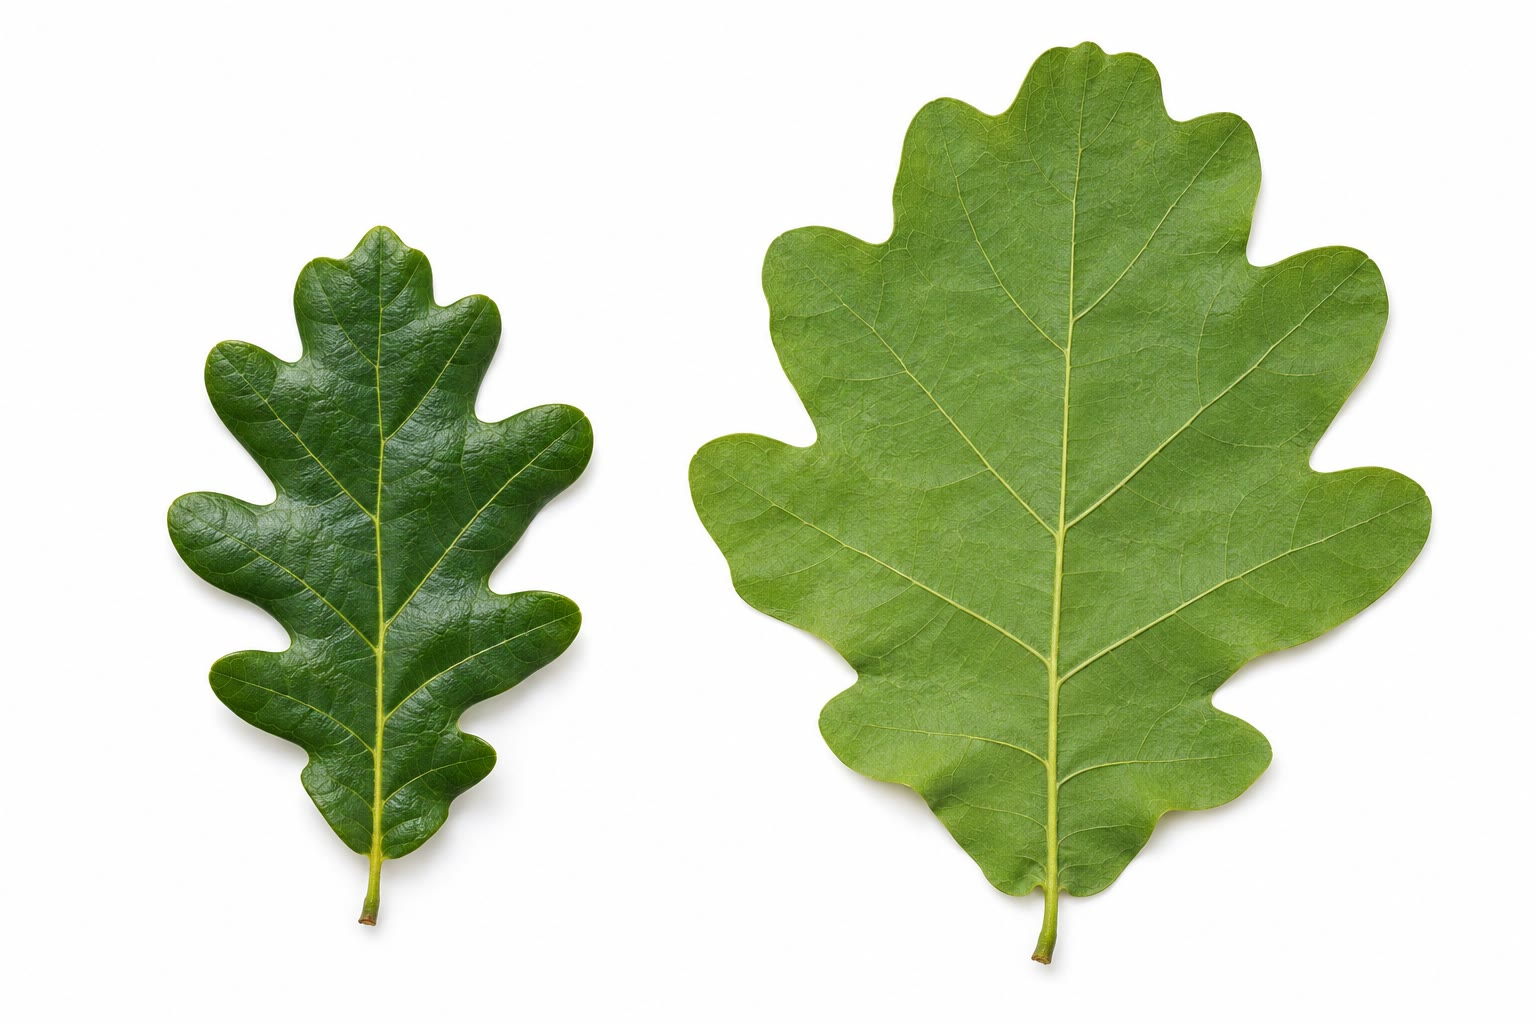
\includegraphics[width=0.55\linewidth]{images/book4/ai/b4-15-sun-shade-leaves.jpg}

{\small Una \omterm{prop:b2:plant-plasticity:sunshade}{hoja de sol} y una \omterm{prop:b2:plant-plasticity:sunshade}{hoja de sombra} de un mismo roble: el mismo
\omterm{def:b2:meiosis-heredity:vocabulary}{genotipo}, distinta luz, distintas hojas.}
\end{omfigure}

\section{Leer la luz}

\begin{theorem}[El fitocromo como medidor de la calidad de la luz]\label{thm:b2:plant-plasticity:phytochrome}
\index{fitocromo}\index{relación rojo/rojo lejano}\index{evitación de la sombra}
El fitocromo existe en dos formas: $P_r$, que absorbe la luz roja
(\qty{660}{nm}) y se convierte en $P_{fr}$, y $P_{fr}$, que absorbe el
rojo lejano (\qty{730}{nm}) y vuelve a la forma inicial --- y es
$P_{fr}$ la forma que actúa. Con luz continua, las dos conversiones se
equilibran en un \emph{fotoequilibrio} cuya posición solo depende de la
relación entre rojo y rojo lejano de la luz:
\[
\varphi = \frac{P_{fr}}{P_{r} + P_{fr}} = \frac{R}{R + a\,FR},
\]
donde $R$ y $FR$ son las densidades de flujo de fotones en las dos bandas
y $a$ una constante del pigmento ($a \approx 0.77$). La luz solar tiene
$R{:}FR \approx 1.15$, lo que da $\varphi \approx 0.6$; la luz filtrada
por las hojas, que absorben el rojo y transmiten el rojo lejano, tiene
$R{:}FR
\approx 0.2$ y $\varphi \approx 0.2$. Un $\varphi$ bajo indica a una
planta que está bajo otras plantas o junto a ellas antes de estar
realmente sombreada --- el rojo lejano reflejado por una vecina se detecta
en el lado que da hacia ella --- y la planta responde con el
\emph{síndrome de \omterm{thm:b2:plant-plasticity:phytochrome}{evitación de la sombra}}: alargamiento más rápido del
tallo, pecíolos más largos, hojas más erguidas, menos ramificación,
floración más temprana. Una plántula bajo un dosel cerrado duplica su
ritmo de alargamiento.
\end{theorem}
\begin{proof}
Sea $k_1 R$ la constante de velocidad de $P_r \to P_{fr}$ (proporcional
al flujo de rojo) y $k_2\,FR$ la de $P_{fr} \to P_r$. En el
equilibrio, $k_1 R\,P_r = k_2\,FR\,P_{fr}$, de modo que $P_{fr}/P_r = k_1 R/
(k_2 FR)$ y $\varphi = P_{fr}/(P_r + P_{fr}) = R/(R + a\,FR)$ con
$a = k_2/k_1$. (Ambas formas absorben algo en las dos bandas, lo que
engloba la constante $a$; la forma del resultado no cambia.) Con
$a = 0.77$: $1.15/(1.15 + 0.77) = 0.60$; $0.2/(0.2 + 0.77) = 0.21$.
\end{proof}

\begin{omfigure}
\begin{tikzpicture}
\begin{axis}[
  width=0.7\linewidth, height=5.2cm,
  axis x line=bottom, axis y line=left,
  xmin=0, xmax=1.4, ymin=0, ymax=0.8,
  xlabel={relación rojo : rojo lejano de la luz}, ylabel={$\varphi = P_{fr}/P_{\text{total}}$},
  xlabel style={font=\small, at={(axis description cs:0.5,-0.13)}, anchor=north},
  ylabel style={font=\small},
  tick label style={font=\small}, xtick={0,0.2,0.6,1.15}, ytick={0,0.2,0.4,0.6},
  clip=false,
]
\addplot[very thick, omDef, domain=0:1.4, samples=60] {x/(x+0.77)};
\draw[dashed, gray] (axis cs:1.15,0) -- (axis cs:1.15,0.6) -- (axis cs:0,0.6); \node[font=\scriptsize, anchor=south west] at (axis cs:1.15,0.6) {pleno sol};
\draw[dashed, gray] (axis cs:0.2,0) -- (axis cs:0.2,0.21) -- (axis cs:0,0.21); \node[font=\scriptsize, anchor=west] at (axis cs:0.25,0.15) {bajo un dosel};
\end{axis}
\end{tikzpicture}

{\small El fotoequilibrio del fitocromo en función de la relación entre
rojo y rojo lejano. La luz solar mantiene la mayor parte del pigmento en
la forma activa; la luz filtrada por las hojas lo mantiene sobre todo
inactivo, y la planta interpreta la diferencia como la presencia de
vecinas.}
\end{omfigure}

\begin{proposition}[El fototropismo]\label{prop:b2:plant-plasticity:phototropism}
\index{fototropismo}\index{tropismo}\index{hipótesis de Cholodny--Went}
Un \emph{tropismo} es un movimiento de crecimiento orientado por un
estímulo direccional. En el \emph{fototropismo}, un tallo se curva hacia
la luz azul: la luz se percibe en el extremo mediante un receptor de luz
azul (la fototropina), la auxina que desciende desde el extremo se desvía
hacia el lado sombreado --- sus transportadores se desplazan a la membrana
lateral ---, y el lado sombreado, que recibe más auxina, se alarga más
deprisa que el iluminado, de modo que el tallo se curva hacia la luz. La
curvatura es crecimiento diferencial, no un músculo: solo se produce en la
\omterm{prop:b2:plant-meristems:ram}{zona de elongación}, tarda una o dos horas y es irreversible. Las raíces,
en las que el mismo exceso de auxina \emph{inhibe} el alargamiento, se
curvan en sentido contrario.
\end{proposition}
\begin{proof}[Evidencia]
Darwin (1880) mostró con coleóptilos de gramíneas que el extremo percibe la
luz y que la zona situada debajo se curva: cubrir el extremo con un
capuchón opaco suprimía la curvatura, cubrir la base con un tubo no, y un
capuchón transparente la dejaba intacta. Boysen-Jensen (1913) cortó el
extremo y lo volvió a colocar con un bloque de gelatina intercalado: la
curvatura persistía, de modo que la señal era una sustancia difusible;
una lámina de mica insertada en el lado sombreado la bloqueaba, y en el
lado iluminado no, de modo que la sustancia descendía por el lado
sombreado. Went (1928) recogió la sustancia en agar a partir de extremos
cortados y observó que un bloque colocado descentrado sobre un coleóptilo
decapitado, en la oscuridad, lo hacía curvarse alejándose del bloque ---
en un ángulo proporcional a la cantidad ---, y, recogiendo agar de las dos
mitades de un extremo iluminado por un solo lado, encontró unos dos
tercios de la auxina en el lado sombreado y un tercio en el iluminado
(Briggs, 1957, con mejores métodos). La redistribución lateral de una
hormona de crecimiento es la \omterm{prop:b2:plant-plasticity:phototropism}{hipótesis de Cholodny--Went}, y se ha
mantenido.
\end{proof}

\begin{omfigure}
\begin{tikzpicture}[every node/.style={font=\scriptsize}, >=stealth]
  \foreach \x/\lab/\cap/\bend in {0/{intacto:\\se curva}/0/1, 2.6/{extremo tapado:\\no se curva}/1/0, 5.2/{base tapada:\\se curva}/2/1, 7.8/{extremo cortado:\\no se curva}/3/0, 10.4/{extremo sobre\\gelatina: se curva}/4/1} {
    \begin{scope}[xshift=\x cm]
      \fill[omExo!30] (-0.7,0) rectangle (0.7,0.2);
      \ifnum\bend=1
        \draw[very thick, omExo!70!black] (0,0.2) -- (0,1.6) .. controls (0,2.3) and (0.5,2.6) .. (0.9,2.8);
      \else
        \draw[very thick, omExo!70!black] (0,0.2) -- (0,3.0);
      \fi
      \ifnum\cap=1 \fill[black] (-0.2,2.7) rectangle (0.2,3.1); \fi
      \ifnum\cap=2 \fill[black] (-0.2,0.2) rectangle (0.2,1.5); \fi
      \ifnum\cap=3 \draw[thick] (-0.3,2.6) -- (0.3,2.6); \fi
      \ifnum\cap=4 \fill[omDef!35] (-0.2,2.55) rectangle (0.2,2.75); \draw[very thick, omExo!70!black] (0.55,2.75) -- (0.9,3.1); \fi
      \node[below, align=center] at (0,-0.15) {\lab};
    \end{scope}
  }
  \node[anchor=east, align=right, omProp!80!black] at (-1.0,2.2) {luz desde\\la derecha $\to$};
\end{tikzpicture}

{\small Los experimentos con coleóptilos. Darwin: el extremo percibe la
luz y la región situada debajo se curva; tapar el extremo lo impide,
proteger la base no. Boysen-Jensen: la señal atraviesa un bloque de
gelatina --- es una sustancia.}
\end{omfigure}

\begin{omfigure}
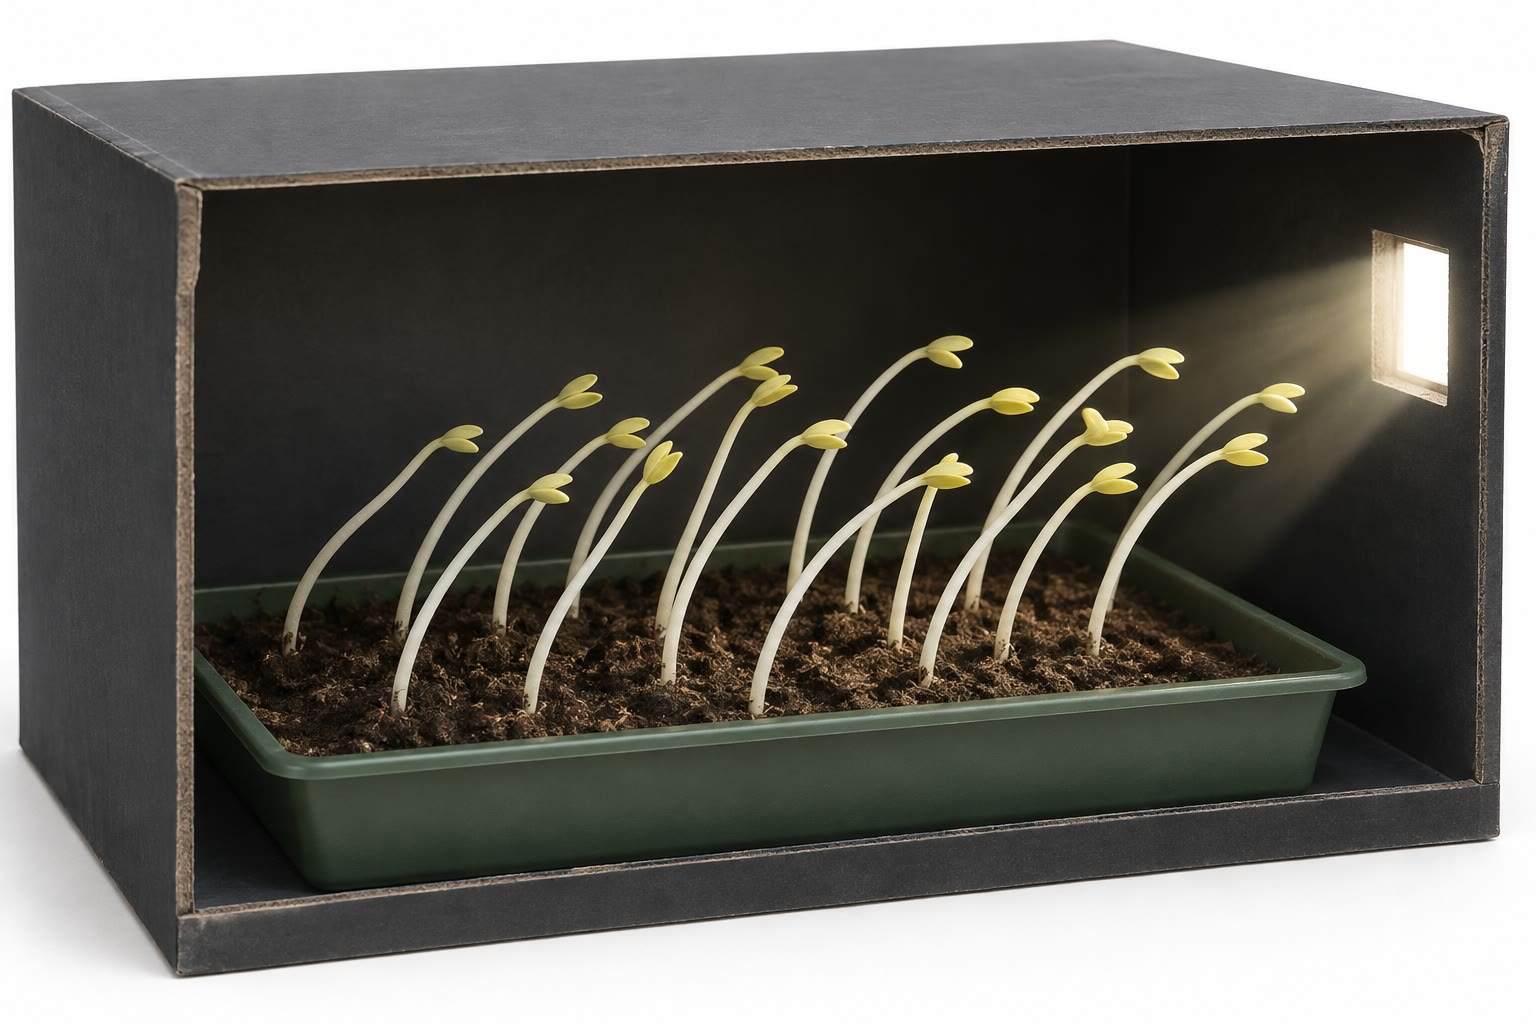
\includegraphics[width=0.55\linewidth]{images/book4/ai/b4-15-phototropism.jpg}

{\small Plántulas en una caja con una sola ventana: todas se curvan hacia la
luz, creciendo más deprisa por el lado opuesto a ella.}
\end{omfigure}

\begin{theorem}[Cuánto se curva un tallo]\label{thm:b2:plant-plasticity:bend}
Si el lado sombreado de un tallo de diámetro $d$ se alarga en una cantidad
relativa $\varepsilon_s$ y el lado iluminado en $\varepsilon_l$ a lo largo
de una zona de crecimiento de longitud $L$, la zona se curva un ángulo
\[
\theta = \frac{L\,(\varepsilon_s - \varepsilon_l)}{d}
\]
(en radianes). Un coleóptilo que crece un \qty{5}{\%} por hora a lo largo
de una zona de \qty{10}{mm} y de \qty{1}{mm} de diámetro, con la auxina
repartida
$65 : 35$ de modo que los dos lados crecen a $1.3$ y $0.7$ veces la media,
se curva en tres horas $\theta = 10\times(0.195 - 0.105)/1 =
0.9$ radianes, unos \qty{50}{\degree}. La curvatura no necesita ningún
mecanismo nuevo: basta el crecimiento ordinario del
\cref{ch:b2:plant-meristems}, desigual en los dos lados.
\end{theorem}
\begin{proof}
Los dos lados de la zona se convierten en arcos de radios $\rho + d/2$ y
$\rho - d/2$ que subtienden el mismo ángulo $\theta$, de longitudes $L(1 +
\varepsilon_s)$ y $L(1 + \varepsilon_l)$; su diferencia es
$\theta d$, de modo que $\theta = L(\varepsilon_s - \varepsilon_l)/d$. En
tres horas a un \qty{5}{\%} por hora el alargamiento medio es $0.15$;
$1.3\times 0.15 = 0.195$ y $0.7\times 0.15 = 0.105$.
\end{proof}

\begin{proposition}[El gravitropismo]\label{prop:b2:plant-plasticity:gravitropism}
\index{gravitropismo}\index{estatolito}
Un tallo tumbado de lado se endereza hacia arriba y una raíz se dirige
hacia abajo en pocas horas. La dirección de la gravedad la perciben los
\emph{estatolitos} --- granos densos de almidón de células especializadas
de la cofia y de la vaina amilífera del tallo ---, que sedimentan en unos
segundos en el lado inferior de la célula y, al presionar sobre la
membrana o el retículo endoplásmico, redirigen los transportadores de
auxina de modo que la auxina se acumula en el lado inferior. En el tallo,
el lado inferior crece más deprisa y el tallo se curva hacia arriba; en
la raíz, el mismo exceso de auxina inhibe el lado inferior, el superior
crece más deprisa y la raíz se curva hacia abajo. Si se elimina la cofia,
la raíz crece recta en cualquier dirección; los mutantes sin almidón
perciben mal la gravedad; una raíz sobre un tambor que gira lentamente
(un clinostato), que nunca deja sedimentar los estatolitos, crece sin
dirección. La respuesta es un segundo uso del mecanismo de
Cholodny--Went, con un sensor distinto.
\end{proposition}

\section{El agua: cerrar los poros}

\begin{proposition}[El control estomático]\label{prop:b2:plant-plasticity:stomata}
\index{estoma}\index{célula oclusiva}\index{ácido abscísico}\index{conductancia estomática}
Los poros de la hoja, los \emph{estomas}, están delimitados cada uno por
dos \emph{\omterm{prop:b2:plant-plasticity:stomata}{células oclusivas}} cuyas paredes están engrosadas de forma
desigual, de modo que cuando captan potasio y agua y se hinchan, se
arquean separándose y abren el poro, y cuando los pierden lo cierran. Se
abren por la mañana con la luz azul y un $\mathrm{CO_2}$ interno bajo, y
se cierran en la oscuridad; se cierran en minutos cuando llega el
\emph{\omterm{def:b2:plant-flowering:dormancy}{ácido abscísico}} --- fabricado en las raíces que perciben la
desecación del suelo y transportado hacia arriba por el xilema, o
fabricado en la propia hoja al perder turgencia --- y cuando el aire está
muy seco. La \emph{\omterm{prop:b2:plant-plasticity:stomata}{conductancia estomática}} $g_s$ fija a la vez el agua
perdida, $E = g_s\,(w_i - w_a)$ (la diferencia de fracción molar de vapor
de agua entre el interior de la hoja, saturado, y el aire), y el
$\mathrm{CO_2}$ captado, $A = g_s\,(c_a -
c_i)/1.6$ (el factor $1.6$ es la razón entre las difusividades del vapor
de agua y del $\mathrm{CO_2}$). La hoja intercambia agua por carbono a
través de una sola válvula, y su \emph{eficiencia en el uso del agua} es
\[
\frac{A}{E} = \frac{c_a - c_i}{1.6\,(w_i - w_a)},
\]
unas milésimas de mol de carbono por mol de agua: una hoja C$_3$ típica
gasta de \qtyrange{400}{600}{g} de agua por gramo de carbono fijado; una
hoja C$_4$, la mitad; una \omterm{prop:b2:plant-plasticity:xerophytes}{planta CAM}, la quinta parte.
\end{proposition}

\begin{omfigure}
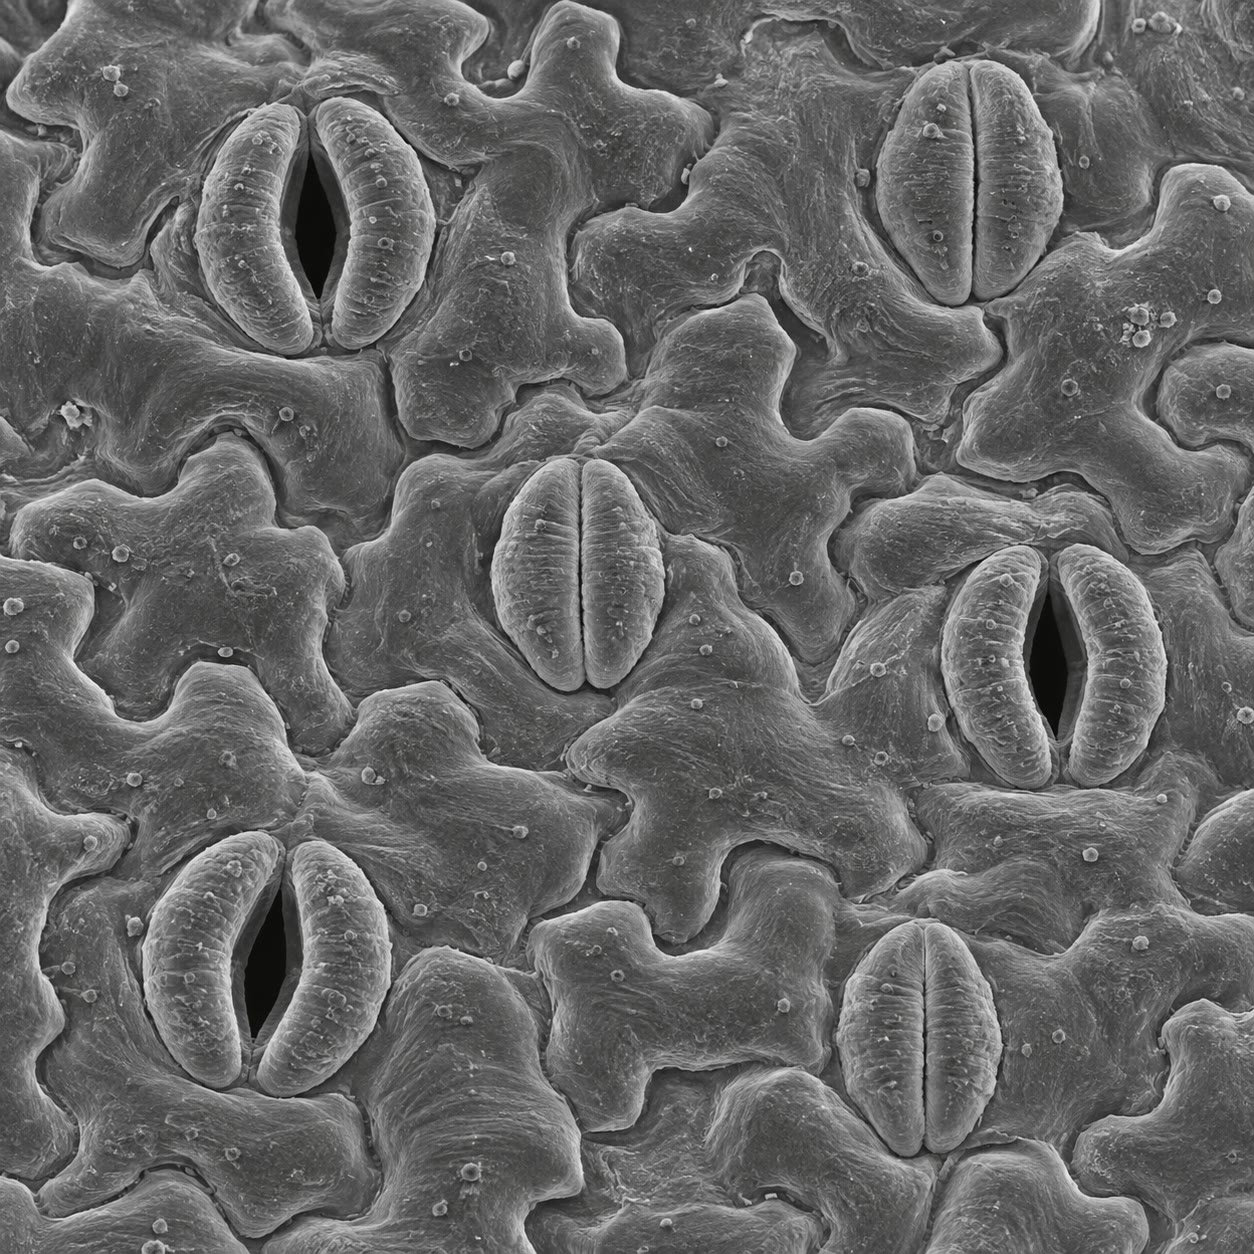
\includegraphics[width=0.42\linewidth]{images/book4/ai/b4-15-stomata-sem.jpg}

{\small Estomas en el envés de una hoja, unos abiertos y otros cerrados:
dos \omterm{prop:b2:plant-plasticity:stomata}{células oclusivas} alrededor de cada poro, la válvula a través de la
cual la hoja intercambia agua por dióxido de carbono.}
\end{omfigure}

\begin{example}[El coste del carbono de un día]\label{ex:b2:plant-plasticity:wue}
A mediodía, una hoja de girasol con $g_s = \qty{0.3}{mol.m^{-2}.s^{-1}}$,
$w_i - w_a = 0.02$ y $c_a - c_i = \qty{120}{\micro mol/mol}$
transpira $E = \qty{6}{mmol.m^{-2}.s^{-1}}$ y fija $A =
0.3\times 120/1.6 = \qty{22}{\micro mol.m^{-2}.s^{-1}}$: $A/E =
\qty{3.7e-3}{}$, es decir, 270 moléculas de agua por cada átomo de
carbono, \qty{400}{g} de agua por gramo de carbono. Una hectárea de esas
hojas pierde \qty{40}{t} de agua en un día de verano para fijar
\qty{100}{kg} de carbono. Cuando el suelo se seca, el \omterm{def:b2:plant-flowering:dormancy}{ácido abscísico}
cierra los estomas hasta una décima parte de esa conductancia: $E$ se
divide por diez, $A$ menos (puesto que $c_i$ también baja), y la planta
sobrevive con una dieta de hambre en lugar de morir de sed.
\end{example}

\begin{proposition}[Adaptaciones a la sequía]\label{prop:b2:plant-plasticity:xerophytes}
\index{xerófito}\index{planta CAM}\index{planta suculenta}
Las plantas de los lugares secos (\emph{xerófitos}) combinan estructuras y
estrategias heredables. Reducir la pérdida: cutícula gruesa, estomas
hundidos en criptas o bajo pelos (que engrosan la capa de aire quieto),
hojas reducidas a espinas (cactus) o que caen en la estación seca, hojas
pequeñas y gruesas que se enrollan. Almacenar: tallos y hojas suculentos
con mucílago que retiene el agua. Alcanzar: raíces de \qty{50}{m} de
profundidad (mezquite) o extendidas justo bajo la superficie para captar
un chaparrón. Desplazar: las \omterm{prop:b2:plant-plasticity:xerophytes}{plantas CAM} abren sus estomas de noche,
cuando $w_i - w_a$ es pequeño, fijan el $\mathrm{CO_2}$ en ácido málico y
lo vuelven a fijar de día con los estomas cerrados --- el mismo carbono
por la quinta parte del agua. Escapar: las anuales del desierto viven como
\omterm{def:b2:angiosperm-reproduction:seed}{semillas} durante años y completan su \omterm{def:b2:plant-life-cycles:cycles}{ciclo de vida} en las semanas
posteriores a la lluvia. Tolerar: las plantas de resurrección pierden el
\qty{95}{\%} de su agua y reviven. Cada estrategia tiene un precio --- el
CAM es lento, la suculencia pesa, las espinas no hacen la fotosíntesis ---,
y la planta que lo paga es superada allí donde el agua abunda.
\end{proposition}

\begin{omfigure}
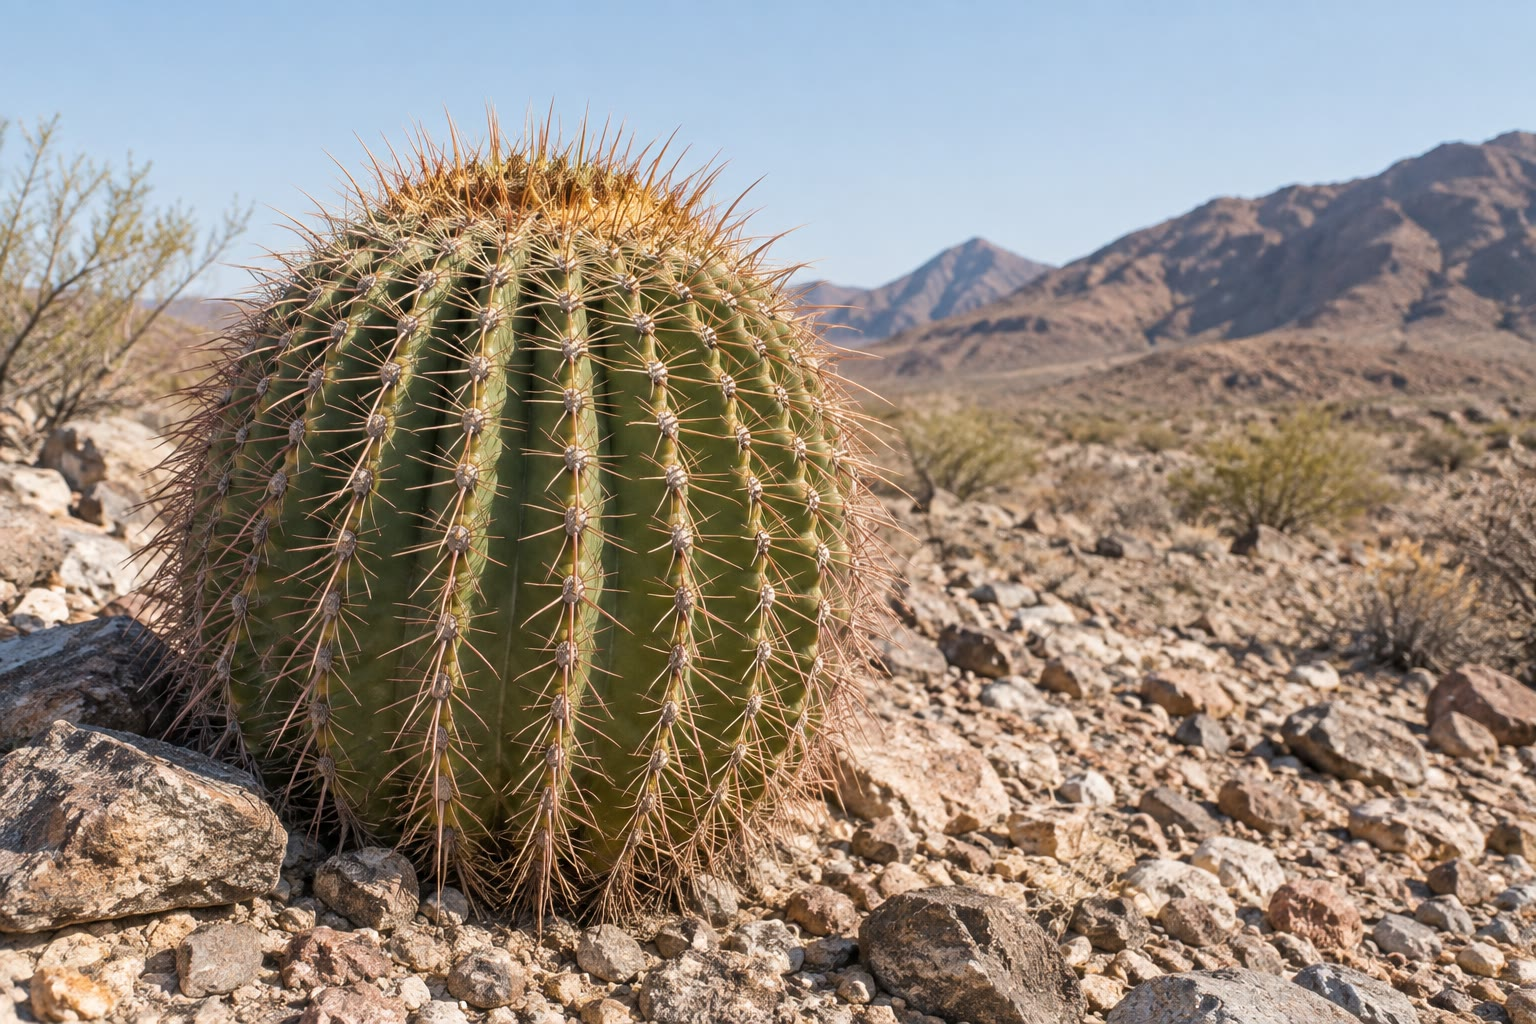
\includegraphics[width=0.55\linewidth]{images/book4/ai/b4-15-cactus.jpg}

{\small Un cactus en forma de barril: un tallo suculento con una cutícula
gruesa, costillas que le permiten hincharse tras la lluvia, hojas
reducidas a espinas y estomas que solo se abren de noche.}
\end{omfigure}

\section{Frío, sal y respuesta al estrés}

\begin{proposition}[La aclimatación al estrés]\label{prop:b2:plant-plasticity:stress}
\index{aclimatación al frío}\index{halófito}\index{proteína de choque térmico}
Una semana a \qty{4}{\celsius} baja la temperatura letal de un centeno de
invierno de \qty{-5}{\celsius} a \qty{-25}{\celsius}: las células han
acumulado azúcares y proteínas que bajan el punto de congelación y
protegen las membranas, han cambiado sus lípidos para mantenerse fluidas
y han fabricado proteínas anticongelantes que impiden crecer a los
cristales de hielo; lo que mata no es el hielo, que se forma sin daño
entre las células, sino la deshidratación de la célula cuando el agua la
abandona para unirse al hielo. Unas pocas horas a \qty{40}{\celsius}
inducen \emph{\omterm{prop:b2:plant-plasticity:stress}{proteínas de choque térmico}} que repliegan las proteínas
desnaturalizadas y protegen la célula a \qty{45}{\celsius}. La sal se
combate con la exclusión en la raíz, la compartimentación en la vacuola
(con solutos compatibles en el citosol para equilibrarla) y, en los
verdaderos \emph{halófitos}, la secreción por glándulas salinas. La
mayoría de estas respuestas pasan por la misma señalización: un sensor,
un aumento del calcio citosólico, el \omterm{def:b2:plant-flowering:dormancy}{ácido abscísico} y un conjunto de
\omterm{prop:b2:cell-differentiation:transcriptional}{factores de transcripción} que activan cientos de genes protectores --- un
programa de estrés tan general como la respuesta inmunitaria de un animal
y, como ella, costoso: la planta aclimatada crece despacio, y una planta
que se aclimata cuando no lo necesita pierde frente a otra que no lo hace.
\end{proposition}
\begin{proof}[Evidencia]
Los experimentos de \omterm{prop:b2:plant-plasticity:stress}{aclimatación al frío} miden la temperatura a la que
mueren la mitad de las células de una hoja (la LT$_{50}$) antes y después
de un periodo a baja temperatura; el desplazamiento, de diez a veinte
grados en una semana, se invierte con una semana de calor. Los mutantes
incapaces de activar el programa del frío (los \omterm{prop:b2:cell-differentiation:transcriptional}{factores de transcripción}
CBF) se aclimatan mal, y las plantas que expresan esos factores de forma
constitutiva sobreviven a las heladas sin \omterm{def:b2:plant-plasticity:plasticity}{aclimatación} --- pero crecen
enanas.
\end{proof}

\begin{omfigure}
\begin{tikzpicture}[every node/.style={font=\scriptsize}, >=stealth]
  \node[draw, rounded corners, fill=omExo!25, align=center] (s) at (0,0) {estrés\\sequía, frío,\\sal, calor};
  \node[draw, rounded corners, fill=omDef!15, align=center] (sen) at (3.2,0) {sensor\\(membrana, turgencia,\\proteínas desplegadas)};
  \node[draw, rounded corners, fill=omDef!15, align=center] (ca) at (6.4,0) {segundos mensajeros\\Ca$^{2+}$, ABA};
  \node[draw, rounded corners, fill=omProp!20, align=center] (tf) at (9.6,0) {factores de\\transcripción};
  \node[draw, rounded corners, fill=omThm!15, align=center] (out) at (12.8,0.9) {genes protectores:\\solutos, anticongelantes,\\chaperonas, transportadores};
  \node[draw, rounded corners, fill=omThm!15, align=center] (out2) at (12.8,-0.9) {crecimiento frenado:\\el coste};
  \draw[->, thick] (s) -- (sen); \draw[->, thick] (sen) -- (ca); \draw[->, thick] (ca) -- (tf);
  \draw[->, thick] (tf) -- (out); \draw[->, thick] (tf) -- (out2);
\end{tikzpicture}

{\small La forma común de la respuesta de una planta al estrés: un sensor,
una señal de calcio y de \omterm{def:b2:plant-flowering:dormancy}{ácido abscísico}, \omterm{prop:b2:cell-differentiation:transcriptional}{factores de transcripción} y un
programa de genes protectores --- pagado con crecimiento.}
\end{omfigure}

\begin{example}[Señales que mienten]\label{ex:b2:plant-plasticity:lie}
La plasticidad solo vale lo que vale la señal. Una plántula bajo la
sombra rica en rojo lejano de una vecina se alarga --- con acierto si la
vecina es una plántula a la que puede superar; fatalmente si es un árbol,
puesto que las reservas gastadas en el tallo se pierden para la raíz y la
hoja. Los cultivos sembrados densos se sombrean entre sí, se alargan y se
encaman; los mejoradores han seleccionado trigos y arroces que ignoran la
señal del rojo lejano. Una semana cálida en febrero hace brotar hojas que
una helada de marzo mata; las plantas que sobreviven son las que también
cuentan el frío (\cref{ch:b2:plant-flowering}). Toda respuesta plástica es
una apuesta sobre la honestidad de la señal, y la \omterm{def:b2:plant-plasticity:plasticity}{norma de reacción} está
moldeada por la frecuencia con que, en el pasado del linaje, la señal
dijo la verdad.
\end{example}

\section{Ejercicios}

\begin{exercise}[$\star$]\label{exo:b2:plant-plasticity:1}
Defínanse \omterm{def:b2:plant-plasticity:plasticity}{plasticidad fenotípica}, \omterm{def:b2:plant-plasticity:plasticity}{norma de reacción}, \omterm{def:b2:plant-plasticity:plasticity}{aclimatación} y
\omterm{def:b2:plant-plasticity:plasticity}{adaptación}, con un ejemplo vegetal de cada una.
\end{exercise}

\begin{exercise}[$\star$]\label{exo:b2:plant-plasticity:2}
Descríbanse los cuatro tratamientos de coleóptilos de Darwin y lo que
mostró cada uno.
\end{exercise}

\begin{exercise}[$\star$]\label{exo:b2:plant-plasticity:3}
Enumérense cinco diferencias entre una \omterm{prop:b2:plant-plasticity:sunshade}{hoja de sol} y una \omterm{prop:b2:plant-plasticity:sunshade}{hoja de sombra},
y dígase en qué momento de la vida de la hoja se toma la decisión.
\end{exercise}

\begin{exercise}[$\star$]\label{exo:b2:plant-plasticity:4}
¿Cómo se abre un estoma, qué lo abre por la mañana y qué lo cierra durante
una sequía?
\end{exercise}

\begin{exercise}[$\star\star$]\label{exo:b2:plant-plasticity:5}
Calcúlese $\varphi$ para $R{:}FR = 1.15$ (sol), $0.7$ (un claro), $0.2$
(bajo un dosel) y $0.05$ (sombra profunda) con $a = 0.77$. ¿Entre cuáles
de estos valores activa la planta la \omterm{thm:b2:plant-plasticity:phytochrome}{evitación de la sombra} si el umbral
es $\varphi = 0.4$?
\end{exercise}

\begin{exercise}[$\star\star$]\label{exo:b2:plant-plasticity:6}
Una hoja tiene $g_s = \qty{0.25}{mol.m^{-2}.s^{-1}}$, $w_i - w_a = 0.025$ y
$c_a - c_i = \qty{100}{\micro mol/mol}$. Calcúlense $E$, $A$, la eficiencia
en el uso del agua en moles y en gramos de agua por gramo de carbono, y el
agua perdida por metro cuadrado en un día de 12 horas.
\end{exercise}

\begin{exercise}[$\star\star$]\label{exo:b2:plant-plasticity:7}
Vuélvase a calcular el ejercicio anterior para una \omterm{prop:b2:plant-plasticity:xerophytes}{planta CAM} cuyos
estomas se abren de noche con $w_i - w_a = 0.005$ y la misma conductancia.
¿En qué factor se reduce el coste en agua del carbono?
\end{exercise}

\begin{exercise}[$\star\star$]\label{exo:b2:plant-plasticity:8}
Un estatolito es un grano de almidón de \qty{2}{\micro m} de radio y
densidad \qty{1500}{kg/m^3} en un citoplasma de densidad
\qty{1100}{kg/m^3} y viscosidad \qty{0.01}{Pa.s}. Calcúlense su velocidad
de sedimentación (Stokes) y el tiempo que tarda en atravesar una célula de
\qty{10}{\micro m}. ¿Por qué un clinostato que gira una vez por minuto
suprime el gravitropismo?
\end{exercise}

\begin{exercise}[$\star\star$]\label{exo:b2:plant-plasticity:9}
Un tallo de \qty{2}{mm} de diámetro crece un \qty{2}{\%} por hora a lo
largo de una zona de \qty{20}{mm}. La luz de un lado reparte la auxina
$60 : 40$. ¿Qué ángulo se ha curvado al cabo de dos horas? ¿Al cabo de
cuánto tiempo forma \qty{90}{\degree} con su dirección inicial?
\end{exercise}

\begin{exercise}[$\star\star\star$]\label{exo:b2:plant-plasticity:10}
Una plántula con \qty{50}{mg} de reservas se alarga \qty{2}{cm} al día al
descubierto y \qty{4}{cm} al día bajo un dosel, y gasta \qty{1}{mg} de
reservas por centímetro de tallo por encima de lo que aportan sus hojas.
El dosel está \qty{30}{cm} por encima de ella en un ortigal y \qty{10}{m}
en un bosque. ¿En qué caso tiene éxito la \omterm{thm:b2:plant-plasticity:phytochrome}{evitación de la sombra}, y qué
ocurre en el otro?
\end{exercise}

\begin{exercise}[$\star\star\star$]\label{exo:b2:plant-plasticity:11}
Explíquese por qué la congelación mata una célula por deshidratación y no
por el hielo, qué hace una semana de frío para impedirlo, y por qué una
planta que expresa el programa del frío todo el año es enana.
\end{exercise}

\begin{exercise}[$\star\star\star$]\label{exo:b2:plant-plasticity:12}
``La plasticidad es una apuesta sobre la honestidad de una señal.''
Discútase a partir de la señal del rojo lejano, de la semana cálida de
febrero y de la mejora de cultivos que ignoran a sus vecinos.
\end{exercise}

\section{Problema: una plántula bajo el dosel}

\begin{problem}[{Problema de fin de semana --- se calculan el clima
luminoso de una plántula, su alargamiento, su balance hídrico y sus
tropismos a partir de la física de sus sensores, hasta llegar a su estado
de fitocromo, su altura al cabo de quince días y su consumo diario de
agua}]
\label{pb:b2:plant-plasticity:1}
Una plántula de abedul germina bajo un dosel que transmite el
\qty{3}{\%} de la luz solar y reduce $R{:}FR$ de $1.15$ a $0.2$
($a = 0.77$). A pleno sol se alargaría \qty{1.5}{cm} al día; bajo el dosel,
su ritmo de alargamiento se multiplica por $1 +
2(0.6 - \varphi)$. Su tallo mide \qty{2}{mm} de diámetro, con una zona de
crecimiento de \qty{15}{mm}. Hojas: \qty{20}{cm^2} en total; $g_s =
\qty{0.2}{mol.m^{-2}.s^{-1}}$; $w_i - w_a = 0.015$ a la sombra y
$0.03$ en un claro; $c_a - c_i = \qty{80}{\micro mol/mol}$; el día dura
\qty{14}{h}. Estatolitos: radio de \qty{2.5}{\micro m}, densidad de
\qty{1500}{kg/m^3}, en un citoplasma de \qty{1100}{kg/m^3} y
\qty{0.01}{Pa.s}.

\medskip
\noindent\textbf{Parte I --- La luz.}
\begin{enumerate}
  \item Calcúlese $\varphi$ al descubierto y bajo el dosel.
  \item ¿Qué concluye la plántula a partir de $\varphi$, y qué concluiría
        si el dosel transmitiera el \qty{3}{\%} de la luz sin cambiar su
        color (una malla de sombreo)?
  \item Calcúlese el ritmo de alargamiento bajo el dosel.
  \item ¿Qué altura tiene la plántula al cabo de 14 días allí, frente a una
        hermana al descubierto?
  \item Se abre un claro a un lado, lo que eleva $R{:}FR$ en ese lado a
        $0.8$. ¿Qué dos respuestas se producen, y mediante qué dos
        fotorreceptores?
  \item ¿Por qué las hojas desarrolladas bajo el dosel son más grandes y
        finas, y qué les ocurre si se tala el dosel?
\end{enumerate}

\medskip
\noindent\textbf{Parte II --- Curvarse hacia el claro.}
\begin{enumerate}[resume]
  \item La luz del claro reparte la auxina $65 : 35$ a través del tallo. Con
        el ritmo de alargamiento bajo el dosel de la pregunta 3, calcúlese
        el alargamiento relativo de cada lado de la zona de crecimiento en
        una hora.
  \item Calcúlese el ángulo de curvatura al cabo de una hora.
  \item ¿Al cabo de cuánto tiempo apunta el tallo directamente al claro,
        si el claro está a \qty{60}{\degree} de la vertical?
  \item El tallo está ahora inclinado. Calcúlense la velocidad de
        sedimentación de un estatolito y el tiempo que tarda en atravesar
        una célula de \qty{12}{\micro m}.
  \item El gravitropismo y el fototropismo del tallo están ahora en
        desacuerdo. ¿Cuál se impone en una planta que evita la sombra, y
        por qué es adaptativo?
  \item Una piedra inclina \qty{45}{\degree} una raíz de la misma
        plántula. Predígase su respuesta y explíquese por qué es opuesta a
        la del tallo aunque el mecanismo sea el mismo.
\end{enumerate}

\medskip
\noindent\textbf{Parte III --- El agua.}
\begin{enumerate}[resume]
  \item Calcúlense la transpiración por metro cuadrado a la sombra y el
        agua que pierden en un día las hojas de la plántula.
  \item Calcúlense el carbono fijado por metro cuadrado por segundo y por
        día, y la eficiencia en el uso del agua en gramos de agua por
        gramo de carbono.
  \item ¿Cuál es la ganancia diaria total de carbono de la plántula a la
        sombra, en miligramos?
  \item Vuélvanse a calcular el agua perdida y la eficiencia en el claro.
  \item El suelo se seca y el \omterm{def:b2:plant-flowering:dormancy}{ácido abscísico} reduce $g_s$ a
        \qty{0.02}{mol.m^{-2}.s^{-1}}. Vuélvanse a calcular $E$ y $A$
        (supóngase que $c_a - c_i$ sube a \qty{200}{\micro mol/mol}).
        ¿Cuál disminuye más, y por qué?
  \item La plántula tiene \qty{5}{g} de tejido foliar con un \qty{85}{\%}
        de agua y puede perder la quinta parte antes de marchitarse.
        ¿Cuánto aguanta en el claro con los estomas abiertos si las raíces
        no aportan nada?
  \item Explíquese por qué una estrategia CAM no le convendría a una
        plántula de abedul bajo un dosel.
\end{enumerate}

\medskip
\noindent\textbf{Parte IV --- La apuesta.}
\begin{enumerate}[resume]
  \item La plántula tiene \qty{100}{mg} de reservas y gasta \qty{2}{mg} por
        centímetro de tallo por encima de lo que aportan sus hojas a la
        sombra. ¿Cuánto tallo puede construir solo con sus reservas?
  \item El dosel es un ortigal situado \qty{40}{cm} por encima; después,
        un bosque situado \qty{8}{m} por encima. Dígase en cada caso si el
        alargamiento alcanza la luz antes de que se agoten las reservas, y
        cuál habría sido la mejor respuesta en el bosque.
  \item El abedul es un pionero de terrenos abiertos; una plántula de haya
        puede esperar décadas en sombra profunda. Compárense sus \omterm{def:b2:plant-plasticity:plasticity}{normas de
        reacción} esperadas frente a $\varphi$.
  \item Un mejorador quiere un cultivo de siembra densa que no se alargue.
        ¿Qué sensor o qué respuesta desactivaría, y qué efecto secundario
        debe comprobar?
  \item Explíquese en dos frases por qué una planta que no puede percibir
        a sus vecinas y una planta que siempre se fía de ellas salen ambas
        peor paradas que una que se fía a veces.
  \item Enúnciese el resultado: $\varphi$ al sol y a la sombra, la altura de
        la plántula al cabo de 14 días y su consumo diario de agua a la
        sombra y en el claro.
\end{enumerate}
\end{problem}
